\section{Quasipolynomial approximations approaching two}
\label{sec:quasipolynomial}

The same construction works for both objectives. A graded schedule
orders adjacent hull blocks with only a small loss in their ranks,
giving a leading factor close to two plus an additive penalty. We then
optimize a short initial part of the tree exactly; this lookahead
absorbs the remaining penalty into the multiplicative factor. The
algorithm returns a completed tree, with its graded recursion
supplying each internal continuation.

\subsection{Algorithm and the three supporting propositions}

Given $0<\varepsilon\le1$, use grade spacing
$\lambda=1+\varepsilon/2$ and write $a=2\lambda$.
The only user-selected parameter is $\varepsilon$. At the end of the
proof, we choose the balance threshold and continuation coefficients
to satisfy the inductive inequalities; these feasible values yield the
stated factor.
\GradeDP\ stores a small number of cumulative rank budgets.
\Rollout\ compares each legal root query with stopping lookahead and
attaching the graded continuation, using the costs of the constructed
trees.

A nearly exact schedule must satisfy several early-rank requirements
at once. The optima for separate coverage budgets can have incompatible
prefixes, so the graded dynamic program retains their compatibility
explicitly.

\begin{proposition}[Graded interval scheduling]
\label{prop:qp-grade-schedule}
For ordinary interval demands with $r$ nested rank budgets at most $B$,
\GradeDP\ decides simultaneous feasibility and returns a schedule in
$(M+1)^{O(r)}(B+1)^{O(r)}$ time, where $M$ is the number of candidates.
Circular demands add enumeration of their first candidate.

For positive demands of weights $w(I)$ and zero-pattern mass $p_0$,
the same DP, with delay levels $0$ and the distinct
$\lfloor\lambda^j\rfloor$, returns an ordering whose
\emph{joint delay cost}
\[
 F(Q)=2\sum_Iw(I)(\operatorname{first}_Q(I)-1)+2p_0|Q|
\]
is at most $\lambda$ times the minimum. It uses
$r=O(\varepsilon^{-1}\log n)$ grades. For rational input weights,
the data-dependent DP entries are sums of weights times integer ranks,
so their bit lengths remain polynomial. The subtraction of one prices
delay before the hitting block; the zero term prices the complete
negative route.
\end{proposition}

Scheduling ranks is only part of identification: endpoint recovery
and later recursive work still cost queries. The next proposition
combines them with restriction credit, leaving a small state potential
as the only additive penalty.

Let $B_W(S)$ be the height and $B_E(S)$ the original-prior expected
depth of the corresponding graded continuation on state $S$. Both
quantities include discovery, endpoint queries, and all recursive child
trees; the continuations return a leaf at singleton states.

\begin{proposition}[Graded continuation bounds]
\label{prop:qp-baselines}
There are fixed balance parameters for which the two graded
continuations, zero on singletons, satisfy
\begin{align}
 B_W(S)&\le a\OPT_W(S)+3\log_2|S|,
       \label{eq:qp-max-induction}\\
 B_E(S)&\le a\OPT_E(S)+4\mathcal E(S).
       \label{eq:qp-expected-ratio}
\end{align}
They use only supplied lines and run in
$(mn)^{O(\varepsilon^{-1}\log n)}$ time, times a polynomial in the
input bit length. The expected-depth bound has no dependence on the
smallest prior.
\end{proposition}

To turn the continuation bound into a multiplicative guarantee, we
optimize an initial prefix. We charge those queries at their realized
cost, and the resulting saving absorbs the remaining penalty.

\begin{proposition}[Lookahead removes a bounded continuation penalty]
\label{lem:lookahead-completion}
Suppose a legal continuation on every restricted state $S'$ obeys
either $B_W(S')\le a\OPT_W(S')+L_W$, or
$B_E(S')\le a\OPT_E(S')+L_Ew(S')$, with $a>1$.
Exact $k$-level lookahead is an $a$-approximation if, respectively,
$k\ge L_W/(a-1)$ or $k\ge L_E/(a-1)$.
The continuation costs at singletons are zero.
\end{proposition}

\begin{algorithm}[H]
\caption{\Rollout: exact initial-tree optimization with a baseline}
\label{alg:rollout}
\KwIn{State $S$, objective $o$, lookahead $j$, and legal baseline routine $B$.}
\KwOut{The cheapest initial tree of at most $j$ levels, completed by $B$.}
\If{$|S|\le1$}{\KwRet its leaf\;}
\If{$(S,o,j)$ is memoized}{\KwRet the stored tree and cost\;}
Compute the actual baseline tree $B(S)$ and retain it as the initial best choice\;
\If{$j>0$}{
  \ForEach{supplied line $\ell$ splitting $S$}{
    Recurse on $S_\ell^-,S_\ell^+$ with lookahead $j-1$\;
    Compare $1+\max\{v_-,v_+\}$ if $o=\mathrm W$,
    or $w(S)+v_-+v_+$ if $o=\mathrm E$, with the best cost\;
    Store a lower-cost choice and its two child trees\;
  }
}
Memoize and return the best choice\;
\end{algorithm}

For Theorem~\ref{thm:qp-two-plus-epsilon}, use Algorithm~\ref{alg:qp-baselines}
with $\lambda=1+\varepsilon/2$ and
$k=\min\{n-1,\lceil3\lceil\log_2n\rceil/(1+\varepsilon)\rceil\}$.
This choice sets the lookahead cap for both objectives; the baseline
completes every search branch that reaches the cap.

\begin{figure}[htbp]
\centering
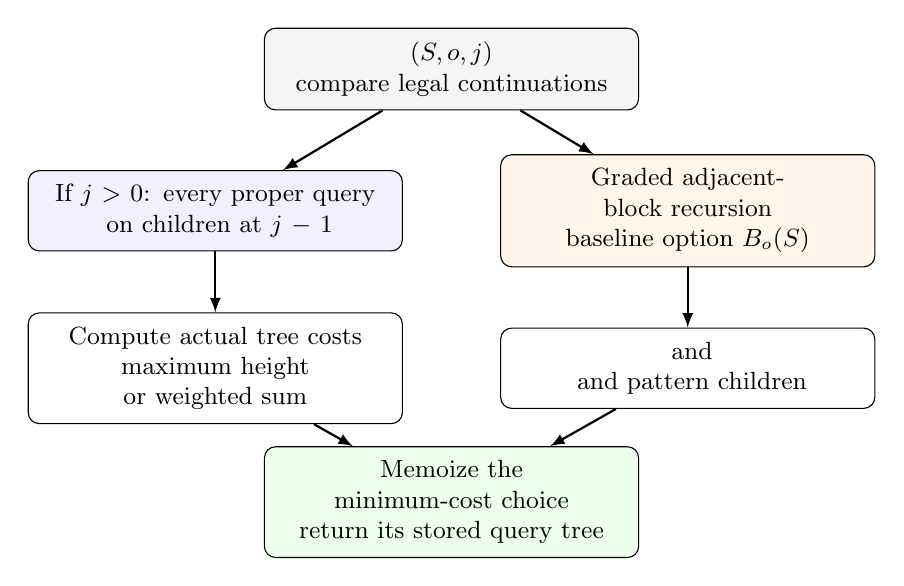
\begin{tikzpicture}[every node/.style={font=\small},
  box/.style={draw,rounded corners,align=center,inner sep=5pt,text width=4.4cm},
  arr/.style={-latex,thick}]
  \node[box,fill=gray!8] (rollout) at (0,0)
    {\Rollout$(S,o,j)$\\compare legal continuations};
  \node[box,fill=blue!6] (split) at (-3,-1.8)
    {If $j>0$: every proper query\\\Rollout\ on children at $j-1$};
  \node[box,fill=orange!8] (baseline) at (3,-1.8)
    {Graded adjacent-block recursion\\baseline option $B_o(S)$};
  \node[box] (grade) at (3,-3.8)
    {\HullData\ and \GradeDP\\\EndpointCode\ and pattern children};
  \node[box] (evaluate) at (-3,-3.8)
    {Compute actual tree costs\\maximum height or weighted sum};
  \node[box,fill=green!7] (best) at (0,-5.5)
    {Memoize the minimum-cost choice\\return its stored query tree};
  \draw[arr] (rollout) -- (split);
  \draw[arr] (rollout) -- (baseline);
  \draw[arr] (baseline) -- (grade);
  \draw[arr] (split) -- (evaluate);
  \draw[arr] (grade) -- (best);
  \draw[arr] (evaluate) -- (best);
\end{tikzpicture}
\caption{Exact lookahead wrapped around the quasipolynomial baseline.
The arrows denote calls and the returned trees or costs. The baseline
completes any branch that reaches its stopping depth. Thus the
logarithmic cap on $j$ bounds the number of search transcripts while
each returned tree still completes identification. The proof compares
this finite search with an optimal tree; the algorithm evaluates only
trees it has constructed.}
\label{fig:qp-procedure-flow}
\end{figure}


\begin{proofstrategy}
\begin{enumerate}
\item Retain several cumulative budgets together. Exact feasibility
      requires nested prefixes, so the graded DP stores their
      compatibility explicitly.
\item Map an optimal witness path to adjacent hull blocks. A query
      already removed by restriction pays for its block delay; a
      count or entropy potential pays for endpoint recovery.
\item Compare lookahead with the first levels of an optimal tree.
      Each paid prefix query replaces a query previously charged at
      factor $a$, which absorbs the continuation penalty.
\end{enumerate}
\end{proofstrategy}

\begin{theorem}\label{thm:qp-two-plus-epsilon}
For every fixed $\varepsilon>0$, maximum depth and
arbitrary-prior expected depth have supplied-query quasipolynomial
$(2+\varepsilon)$ approximations. For $0<\varepsilon\le1$, their time is
\[
(mn)^{O(\varepsilon^{-1}\log n)}
\]
times a polynomial in the
input bit length.
\end{theorem}
\begin{proof}
Use the continuations of Proposition~\ref{prop:qp-baselines} with
$a=2+\varepsilon$. Their penalties on any restricted state are at
most $3\log_2n$ and $4w(S')\ln n$, respectively: $|S'|\le n$
bounds the count potential, and entropy on $|S'|$ hypotheses is at
most $\ln|S'|$ per unit mass. Proposition~\ref{lem:lookahead-completion}
therefore removes both penalties after $O(\log n)$ levels. Concretely, the
final calibration permits
\[
 q_n=\lceil\log_2n\rceil,\qquad
 k=\min\{n-1,\lceil3q_n/(1+\varepsilon)\rceil\}.
\]
When the cap is $n-1$, every proper identifying tree is available,
so the result is exact. Otherwise the lookahead guarantee applies.
At depth $i\le k$, there are at most $2^i$ answer transcripts, and
each transcript is generated by at most $m^i$ choices of supplied
queries along its path. Summing these bounds over $i\le k$ gives
$(2m)^{O(k)}$ lookahead states. Multiplying by the graded-continuation
cost preserves the stated time. For
$\varepsilon>1$, use the construction with $\varepsilon=1$.
\end{proof}

\subsection{Proofs of the supporting propositions}

\subsubsection{Graded schedules retain compatible prefixes}

Each grade prefix has two obligations: stay within its rank budget and
hit every interval whose deadline it represents. Counts enforce the
first; the last selected position suffices to check the second.

\begin{claim}[Counts and last positions decide every interval deadline]
\label{clm:qp-prefix-state}
For each grade prefix $j$, store its selected count $c_j$ and last
selected position $p_j$. When a demand $[l,q]$ ends, it has been
hit within that grade exactly when $p_j\ge l$.
\end{claim}
\begin{proof}
Scan the candidates in spatial order. Selecting position $q$ at
grade $i$ increments $c_j$ and replaces $p_j$ by $q$ for every
$j\ge i$; skipping changes neither. These are exactly the cumulative
counts and last positions. No selected position exceeds the scanned
endpoint $q$, so $p_j\ge l$ is equivalent to a hit in $[l,q]$.
Reject any count exceeding its budget. Sorting the selected
candidates by grade therefore meets every deadline.

Conversely, write the cumulative budgets as $b_j$ and take any
feasible comparison ordering. Drop candidates whose ranks exceed
the last budget; no required deadline hit is lost. Assign each
remaining candidate $v$ the grade
\[
 \operatorname{grade}(v)
   =\min\{j:\operatorname{rank}(v)\le b_j\}.
\]
The candidates with grade at most $j$ are exactly those with
original rank at most $b_j$, so their count is at most $b_j$.
Every demand with deadline $j$ has one such candidate in its
interval. At its right endpoint the last selected position of
that prefix is therefore at least its left endpoint. Thus all
count and hit checks pass, proving the converse. The recurrence
is exact, with at most
$(M+1)^r(B+1)^r$ states and $r+1$ transitions per position.
For circular demands, force the first candidate, delete its hit
demands and cut there. Its absolute rank consumes one unit of
\emph{every} cumulative capacity, including the total-count cap.
\end{proof}

Independent prefix coverage would be insufficient. For example,
$[1,2]$ and $[2,3]$ can both be hit by rank one, while
$\{1\}$ and $\{3\}$ can both be hit by rank two. The first
requirement forces candidate 2 first, leaving too few ranks for the
second. The DP stores exactly this compatibility information.

Exact deadline feasibility must now become an approximation for delay.
Charging the first qualifying grade bounds each positive delay, while
the final selected count also prices the complete negative route.

\begin{claim}[Rounded delays bound the joint objective]
\label{clm:qp-rounded-delay}
Charging a demand at its earliest selected grade gives a
$\lambda$ approximation for $F$, including zero-pattern waiting.
\end{claim}
\begin{proof}
Let $d_0=0$ and let the positive $d_j$ be the distinct
$\lfloor\lambda^j\rfloor$ up to a level covering $n$. Grade $j$
has capacity $d_j+1$. At the right endpoint of demand $I$, charge
$2w(I)d_j$ for the least $j$ whose last selected position lies in
$I$. Its actual first-cover delay is at most $d_j$. Keep the least
accumulated charge for each state, and add $2p_0c_{\rm last}$ at
completion.

For a comparison order, rank one uses grade zero. At rank $t\ge2$,
the first positive level at least $t-1$ is smaller than
$\lambda(t-1)$: the preceding unrounded power is less than the
integer $t-1$. Duplicate-floor plateaus do not change this argument.
These assigned grades respect every cumulative capacity, so
Claim~\ref{clm:qp-prefix-state} makes this graded comparison feasible.
For each positive delay, its rounded charge is at most $\lambda$
times its original charge; the final selected count, and therefore
the zero waiting charge, is unchanged. Since that waiting charge is
nonnegative and $\lambda\ge1$, the minimum surrogate is consequently
at most $\lambda F$. Conversely, the actual delay of each returned
demand is at most its charged grade level, so its actual objective
is no larger than the minimized surrogate.
An optimum uses at most the number of demands, after unproductive
candidates are removed. For a circular order the forced first
candidate has zero delay, all capacities decrease by one, and the
final waiting charge is $2p_0(1+c_{\rm last})$.
\end{proof}

\begin{algorithm}[H]
\caption{\GradeDP: cumulative-grade interval feasibility or weighted delay}
\label{alg:grade-dp}
\KwIn{Ordinary intervals; $r$ capacities $b_0<\cdots<b_{r-1}$;
feasibility deadlines, or weights, delay levels $d_j=b_j-1$,
and zero-pattern mass $p_0$.}
\KwOut{A feasible graded selection, or a minimum surrogate-delay selection.}
Initialize the state $(c_0,\ldots,c_{r-1};s_0,\ldots,s_{r-1})$ to all zeros,
with cost zero; all other states are unreachable\;
\For{$q=1,\ldots,M$}{
  From each reachable state, try skipping $q$ or selecting it at grade $i$\;
  A grade-$i$ selection increments $c_j$ and sets $s_j=q$ for all $j\ge i$\;
  Reject any transition with $c_j>b_j$\;
  \ForEach{interval $I=[l,q]$ ending here}{
    \eIf{mode is feasibility}{
      Reject if $s_j<l$ for its deadline grade $j$\;
    }{
      Find the least $j$ with $s_j\ge l$; reject if none\;
      Add $2w(I)d_j$ to this transition's cost\;
    }
  }
  Keep one feasible witness, or the minimum cost, for each resulting state\;
}
In weighted mode add $2p_0c_{r-1}$ to each final state's cost\;
Reconstruct a winning selection and order it by grade\;
\KwRet the selection and schedule, or infeasible\;
\end{algorithm}

For circular demands enumerate the forced first candidate, remove
its demands, cut there, and reduce \emph{every} capacity by one.
Residual expected costs still use the original delay levels and add
$2p_0(1+c_{r-1})$ at completion. In maximum-depth mode append a final
grade with the total-count cap if it is not already a capacity.
Section~\ref{sec:quasipolynomial} proves the state invariant and
the $(M+1)^{O(r)}(B+1)^{O(r)}$ bound.


\subsubsection{Restriction pays for a graded pattern stage}

For the expected-depth calculations, use the pattern partition $\Pi$
and abbreviate $\Delta=\Delta_{\mathrm E}(S,\Pi)$,
$I=I(S,\Pi)$, $w=w(S)$, and $b=w-w(A_0)$.
Write $J$ for the state-mass-weighted entropy of the actual discovery
transcript, and $W$ for the expected cost of this stage's queries,
before attaching the recursive child trees.

A block rank must be translated back into real queries. The next claim
combines the two possible discovery exits with endpoint recovery;
the second exit benefits from the cached negative first endpoint.

\begin{claim}[An adjacent block has a uniform endpoint allowance]
\label{clm:qp-block-allowance}
If a class $A$ first meets block $k$, its discovery and endpoint
queries use at most
\begin{equation}\label{eq:qp-block-allowance}
 2(k-1)+z_A+5,\qquad
 z_A=\lfloor\log_2(\delta|S|/|A|)\rfloor
\end{equation}
on each route. For expected depth, the analogous overhead is at most
five times the nonzero-pattern mass, plus the pattern information
remaining after discovery.
\end{claim}
\begin{proof}
At most $2(k-1)$ endpoint queries precede the hitting block. A first
endpoint positive costs one query and has endpoint allowance
$z_A+4$ by Proposition~\ref{lem:endpoint-height}. A second endpoint positive costs two queries but has a
cached negative neighbor, reducing its allowance to $z_A+2$.
Thus the two total allowances are respectively
\[
 2(k-1)+1+(z_A+4)=2(k-1)+z_A+5,
\]
\[
 2(k-1)+2+(z_A+2)=2(k-1)+z_A+4.
\]
Their maximum is the stated common allowance.
A block containing the free origin has one real endpoint and obeys
the first bound. For expected depth, the two endpoint-code overheads
are four on the first exit and two on the pinned second exit.
Together with discovery this gives respectively five and four queries
beyond the block delay and the conditional entropy cost. Summing over
positive exits bounds this overhead by $5b$. If $P$ is the pattern
label and $D_{\rm disc}$ the discovery transcript, the latter is a
function of $P$: at this fixed state every discovery query is a hull
test, and all choices and stopping rules depend only on earlier hull
answers. Hence $H(D_{\rm disc}\mid P)=0$, and the entropy chain rule
of Lemma~\ref{lem:entropy-chain-rule} gives
\[
 wH(P\mid D_{\rm disc})=wH(P)-wH(D_{\rm disc})=I-J.
\]
Thus the remaining entropy invoice is $(I-J)/\ln2$. The second
exit's smaller allowance is precisely the negative-neighbor saving.
\end{proof}

For maximum depth, build all pattern-child codes first. For a trial
height $H$, set
\[
 B_A=\left\lfloor\frac{H-B_W(A)-z_A-5}{2}\right\rfloor.
\]
Reject negative budgets. Round each budget down to a delay level,
use block deadline $\widehat B_A+1$, and cap the total selected
blocks at $\lfloor H/2\rfloor$. Enumerate the first block and apply
\GradeDP. The trial range ends at
$\lceil(a+3)(|S|-1)\rceil$. Low-dimensional hulls use their direct
extreme tests.

The computed deadlines use actual child heights, so their feasibility
requires care with integer rounding. Restriction supplies the needed
rank credit before the deadline is rounded down to a grade.

\begin{claim}[Downward rounding retains every required integer rank]
\label{clm:qp-rounded-rank}
At $H^*=\lfloor aD+\gamma\log_2s\rfloor$, where
$D=\OPT_W(S)$ and $s=|S|$, every comparison class is hit by its
computed deadline, provided
\begin{equation}\label{eq:qp-max-parameters}
 \gamma\log_2(1/(1-\delta))\ge1,\qquad
 \gamma\log_2(1/\delta)\ge5,\qquad \gamma\ge1.
\end{equation}
\end{claim}
\begin{proof}
Write $t=t_A$, $x=\log_2(s/|A|)$ and
$u_\delta=\log_2(1/\delta)$. Proposition~\ref{lem:height-prefix} gives
$\OPT_W(A)\le D-(t-1)$. Set
$R_A=a\OPT_W(A)+\gamma\log_2|A|$.
Induction and the integrality of the constructed child height imply
$B_W(A)\le\lfloor R_A\rfloor$, while $z_A=\lfloor x-u_\delta\rfloor$.
Applying $\lfloor u\rfloor-\lfloor v\rfloor\ge\lfloor u-v\rfloor$
twice gives the following chain. The first step uses the inductive
child bound; the second takes the difference of the parent and child
potentials inside one floor; and the third uses the supporting-prefix
credit before taking the second floor difference:
\[
\begin{aligned}
 H^*-B_W(A)-z_A-5
 &\ge\lfloor aD+\gamma\log_2s\rfloor
             -\lfloor R_A\rfloor-\lfloor x-u_\delta\rfloor-5\\
 &\ge\lfloor a(D-\OPT_W(A))+\gamma x\rfloor
             -\lfloor x-u_\delta\rfloor-5\\
 &\ge\lfloor a(t-1)+(\gamma-1)x+u_\delta\rfloor-5.
\end{aligned}
\]
Because $|A|<\delta s$, we have $x>u_\delta$.
The conditions $\gamma\ge1$ and $\gamma u_\delta\ge5$ therefore give
$(\gamma-1)x+u_\delta\ge5$. Hence the last line is at least
$\lfloor a(t-1)+5\rfloor-5=\lfloor a(t-1)\rfloor$.
Dividing the integer credit by two yields
\[
 B_A\ge\left\lfloor\frac{\lfloor a(t-1)\rfloor}{2}\right\rfloor
       =\lfloor\lambda(t-1)\rfloor.
\]
The equality uses $a=2\lambda$ and
$\lfloor\lfloor v\rfloor/2\rfloor=\lfloor v/2\rfloor$.
For $t=1$, level zero suffices. Otherwise choose the last exponent
$j$ with $\lfloor\lambda^j\rfloor\le B_A$, including duplicate
floors. Maximality implies
$\lambda^{j+1}\ge B_A+1>\lambda(t-1)$, so
dividing by $\lambda>0$ gives $\lambda^j>t-1$.
Since $t-1$ is an integer,
$\widehat B_A=\lfloor\lambda^j\rfloor\ge t-1$.
Rounding a real expression before using
this integer credit would not give that conclusion.

Map the optimal witness path to incident hull edges. Each class is
hit by rank at most $t_A$; append an incident edge for an uncovered
terminal nonzero singleton. The comparison uses at most $D$ blocks
when the zero pattern exists, and at most $D+1$ otherwise. The final
calibration ensures $\gamma\log_2s\ge2$ for $s\ge2$.
Since $a\ge2$ and $D$ is an integer,
\[
 H^*=\lfloor aD+\gamma\log_2s\rfloor\ge2D+2,
 \qquad \lfloor H^*/2\rfloor\ge D+1.
\]
The comparison therefore meets the total cap.
Proposition~\ref{prop:qp-grade-schedule} now supplies a passing trial,
and Claim~\ref{clm:qp-block-allowance} bounds every positive route by $H^*$.
The cap also bounds the full negative route, which uses at most
$2\lfloor H^*/2\rfloor\le H^*$ actual tests.
At a balanced state, each child $A$ has
$|A|\le(1-\delta)s$ and $\OPT_W(A)\le D$ by
Lemma~\ref{lem:restriction}. Substituting these two inequalities into
the inductive child bound gives
\[
 1+B_W(A)
 \le aD+\gamma\log_2s
           +1-\gamma\log_2\frac1{1-\delta}
 \le aD+\gamma\log_2s.
\]
The last inequality is exactly the first condition in
\eqref{eq:qp-max-parameters}. For a low-dimensional hull, at most
two extreme tests identify the pattern. Each nonzero class
satisfies $|A|<\delta s$, giving
\[
 2+B_W(A)\le aD+\gamma\log_2s+2-\gamma u_\delta
             \le aD+\gamma\log_2s.
\]
Here the final step uses $\gamma u_\delta\ge5$, so the count-potential
drop pays for both extreme tests.
The zero route ends at its singleton after at most two tests and
also meets the bound because $D\ge1$ and $a\ge2$.
This proves the maximum-depth continuation bound.
\end{proof}

For expected depth, the same witness comparison is summed with the
original hypothesis weights. Discovery information then pays for the
endpoint allowance, giving a local bound that cancels through recursion.

\begin{claim}[Weighted delay and discovery information bound the expected stage]
\label{clm:qp-expected-stage}
The graded expected-depth stage satisfies
\[
 W\le2\lambda\Delta+5b+(I-J)/\ln2,\qquad
 J\ge b\sigma(\delta).
\]
\end{claim}
\begin{proof}
The witness-edge order hits class $A$ by rank $t_A$. When the zero
class exists, its length is at most the witness-path length. Thus
the restriction-credit proposition gives
\[
\begin{aligned}
 F(Q_{\rm wit})
 &=2\sum_{A\ne A_0}w(A)(\operatorname{first}_{Q_{\rm wit}}(A)-1)
     +2p_0|Q_{\rm wit}|
 \\
 &\le2\sum_{A\ne A_0}w(A)(t_A-1)+2p_0\ell\\
 &\byref{Prop.}{lem:support-prefix}{\le}2\Delta.
\end{aligned}
\]
Without the zero class, an
appended terminal singleton has its index $t_A=\ell+1$ and no
waiting term, so the same positive-delay inequality applies.
Claim~\ref{clm:qp-rounded-delay} gives $F(Q_{\rm alg})\le\lambda F(Q_{\rm wit})
\le2\lambda\Delta$.

Adding the allowance of Claim~\ref{clm:qp-block-allowance} yields the
first asserted stage inequality. To bound its information credit, the actual discovery transcript's
positive cells each lie in one vertex cap, even though a comparison
block can meet two caps. Claim~\ref{lem:capped-discovery-entropy} therefore gives
$J\ge b\sigma(\delta)$. Apply Proposition~\ref{lem:stage-conversion} with
$A=2\lambda$ and $B=5$. To see the absorption explicitly,
$ch(\delta)\ge1$ and $h(\delta)\le\ln2$ imply $c\ge1/\ln2$.
Since $0\le J\le I$,
\[
 cI-\frac{I-J}{\ln2}
 =cJ+\left(c-\frac1{\ln2}\right)(I-J)
 \ge cJ\ge cb\sigma(\delta)\ge5b.
\]
In this chain, the first inequality discards the nonnegative term
$(c-1/\ln2)(I-J)$, the second uses the capped-discovery entropy
bound, and the last uses $c\sigma(\delta)\ge5$. Consequently
$W\le a\Delta+cI$.
At a mass-balanced split with relative child mass
$v\in[\delta,1-\delta]$, the query costs $w$ and
$I=wh(v)\ge wh(\delta)$. Thus $cI\ge w$; the nonnegative
restriction decrement permits $w\le a\Delta+cI$ there as well.
Proposition~\ref{prop:potential-cancellation} now adds these local
inequalities over the recursion and cancels every nonroot
optimal-cost and entropy term, giving
$B_E(S)\le a\OPT_E(S)+c\mathcal E(S)$.
The final calibration permits $c=4$.
For a hull of dimension at most one, direct extreme testing costs at
most $2w$. If $p_0>0$, its nonempty zero witness path gives
$\Delta\ge p_0$, so $2w\le2\lambda\Delta+5b$.
Indeed $2w=2p_0+2b\le2\lambda p_0+5b
\le2\lambda\Delta+5b$, since $\lambda\ge1$.
If $p_0=0$, $2w=2b\le5b$. Thus the same stage bound covers the
degenerate branch without invoking the graded DP.
\end{proof}

\begin{algorithm}[H]
\caption{Internal graded continuation for the quasipolynomial algorithm}
\label{alg:qp-baselines}
\KwIn{State $S$; objective $o$; rational $\lambda>1$; fixed balance threshold $1/4$.}
\KwOut{The baseline tree of Section~\ref{sec:quasipolynomial}.}
Stop at a singleton; at a balanced state query a balanced line and recurse\;
At a flat state compute $\HullData(S)$ and use full-hull edges as blocks\;
Handle a hull of dimension at most one by its direct extreme tests\;
\eIf{$o=\mathrm W$}{
  Build the pattern children once and record their heights $C_W(A)$\;
  \For{trial heights $H$ in increasing order}{
    Compute $B_A=\lfloor(H-C_W(A)-z_A-5)/2\rfloor$; reject negative budgets\;
    Round each down to the last level in $\{0\}\cup\{\lfloor\lambda^j\rfloor\}$ not exceeding it\;
    Use deadlines $\widehat B_A+1$ and total cap $\lfloor H/2\rfloor$
    in circular $\GradeDP$; stop at the first feasible trial\;
  }
}{
  Use distinct levels $d_0=0$, $d_j=\lfloor\lambda^j\rfloor$ through a level covering $n$\;
  Minimize the circular weighted-delay surrogate with capacities $d_j+1$
  by $\GradeDP$ and zero-pattern mass $w(A_0)$\;
}
Execute the selected blocks, use pointwise endpoint codes for $\mathrm W$
or expected endpoint codes for $\mathrm E$, and attach recursive pattern children\;
Identify the zero singleton after the negative cover if present; omit it otherwise\;
\KwRet the contracted tree\;
\end{algorithm}

The maximum-depth trial range is
$1\le H\le\lceil(2\lambda+3)(|S|-1)\rceil$.
The baseline selects its trial from these explicit tests, while the
optimum appears in the comparison argument.


There are $O(\varepsilon^{-1}\log n)$ grades, with polynomially many
counts and spatial positions. To compute $z_A$, compare $2^z|A|$
with $\delta|S|$ and choose the largest admissible integer $z$;
this locates the grade directly, without evaluating a logarithm.
All objectives
are rational sums of actual costs. Proper disjoint-child recursion
has at most $n-1$ stages. This proves the time and legality parts of
Proposition~\ref{prop:qp-baselines}.

\subsubsection{Paid prefix queries absorb continuation penalties}

To analyze lookahead, compare with a prefix of an optimal tree. On
every unfinished maximum-depth route, the prefix has already consumed
exactly the queries that create the saving against factor~$a$.

\begin{claim}[The maximum-depth penalty is paid on every frontier path]
\label{clm:lookahead-height-payment}
An optimal height-$D$ tree, truncated at depth $k$, has continuation
height at most $D-k$ at each surviving frontier state.
\end{claim}
\begin{proof}
If $D<k$, the whole optimal tree is a lookahead candidate. Otherwise
each surviving frontier state has optimal height at most $D-k$:
the original optimal subtree is a feasible tree of that height.
The assumed continuation bound therefore completes its path at height
at most
\[
 k+a(D-k)+L_W=aD-(a-1)k+L_W\le aD.
\]
The equality isolates the saving of $a-1$ per paid prefix query, and
the inequality uses $(a-1)k\ge L_W$. Earlier leaves are already
within height $D$. Exact lookahead can only improve this candidate.
\end{proof}

The expected-depth comparison needs no common leaf depth. Only the
mass still unfinished matters: each such hypothesis has paid all
prefix queries, so their total payment absorbs its continuation penalty.

\begin{claim}[Expected prefix cost pays for every surviving frontier mass]
\label{clm:lookahead-expected-payment}
Let $P$ be an optimal tree's expected cost through depth $k$, and
$M_k$ the mass still requiring continuation there. Then $P\ge kM_k$.
\end{claim}
\begin{proof}
Every surviving hypothesis has paid for all $k$ prefix queries.
If $R$ is the sum of the optimal continuation costs, then
$P+R=\OPT_E(S)$ by partitioning the optimal tree's queries at depth
$k$. At each frontier state its optimal restricted cost is no larger
than that of the original subtree, by Lemma~\ref{lem:restriction}.
Thus completing the frontier with the baseline costs
at most
\[
 P+aR+L_EM_k
 =a\OPT_E(S)-(a-1)P+L_EM_k
 \overset{P\ge kM_k}{\le}
 a\OPT_E(S)+[L_E-(a-1)k]M_k.
\]
This is at most $a\OPT_E(S)$ under the stated condition. It assumes
neither a bound on the optimal tree's height nor a lower bound on
its prior masses. These two claims prove the lookahead proposition.
\end{proof}

\subsection{A simple calibration; no optimization is needed}

\begin{parameterchoice}
Fix the balance threshold at $\delta=1/4$, the count coefficient at
$\gamma=3$, and the entropy coefficient at $c=4$. These values
affect only the continuation penalty and lookahead length, which
disappear from the final ratio. Thus no table of optimized constants
is needed for this scheme.
\end{parameterchoice}

Indeed, $(4/3)^3>2$ and $3\log_2 4=6>5$ verify
\eqref{eq:qp-max-parameters}. Here $\sigma(1/4)=\ln4$ and
$h(1/4)\ge\tfrac12\ln2$. The elementary bounds
$2/3\le\ln2<3/4$ give $4h(1/4)>1$ and
$4\sigma(1/4)>5$. The lower bound follows from the first term of
the logarithm series in \eqref{eq:rational-log-bounds}; the upper
bound is the strict trapezoidal bound for $\int_1^2 dx/x$.
Finally $4\ln n<3\log_2 n$, so the single rational lookahead
cap in the theorem covers both objectives. For singleton inputs,
all procedures return the zero-query leaf.
